\documentclass[usenames,dvipsnames]{beamer}
\usepackage{graphicx}
\usepackage{tablefootnote}
\usepackage{bm}
\usepackage{amsmath}
\usepackage{subcaption}
\usepackage{csquotes}
\usepackage[many]{tcolorbox}
\usepackage{listings}
\usepackage{hyperref}
\usepackage{verbatim}
\usepackage[]{textpos}
\usepackage{ragged2e}
\usepackage{dirtytalk}
\usepackage{makecell}
\usepackage{arydshln}

\renewcommand{\emph}[1]{\textbf{#1}}
% This document as well as the corresponding figures were created by
% Mirko Myllykoski, Senior Research Engineer at CS/HPC2N, Umeå
% University, for the January 2021 version of the "Introduction to
% HPC2N" course. 

\beamertemplatenavigationsymbolsempty

\setbeamertemplate{footline}[frame number]

\title{Introduction to HPC2N, Kebnekaise and HPC}
\author{
Birgitte Brydsö, \\
Pedro Ojeda May,
and others at HPC2N}
\institute[Ume{\aa} University]{
  HPC2N \\
  Ume{\aa} University}
\date{19. January 2022}

\titlegraphic{
 \centering
 
\includegraphics[height=0.9cm]{figures/SNIC_logo_lower.png}\;\;\;
 
\includegraphics[height=1.2cm]{figures/umu-logotyp-EN.png}\;\;\;
 
\includegraphics[height=0.9cm]{figures/hpc2n-logo-text5.png}
}

\addtobeamertemplate{frametitle}{}{%
\begin{textblock*}{100mm}(-8mm,83mm)
 
\includegraphics[height=4mm]{figures/umu-logo-left-EN.png}
 
\includegraphics[height=4mm]{figures/SNIC_logo_lower.png}
 
\includegraphics[height=4mm]{figures/hpc2n-logo-text5.png}
\end{textblock*}}

\begin{document}

\frame{
\maketitle
}

\frame{
\frametitle{HPC2N (HPC2N at a glance)}
\begin{itemize}
 \item \emph{High Performance Computing Center North (HPC2N)} is a national center for Scientific and Parallel Computing
\end{itemize}
\begin{center}
 
\includegraphics[width=0.4\textwidth]{figures/hpc2n-logo-text5.png}
\end{center}
\begin{itemize}
 \pause \item A part of \emph{Swedish National Infrastructure for Computing (SNIC)}
\end{itemize}
\begin{center}
 
\includegraphics[height=10mm]{figures/SNIC_logo_lower.png}
\end{center}
}

\frame{
\frametitle{HPC2N (HPC2N at a glance)}

Provides state-of-the-art resources and expertise:
\begin{itemize}
 \item Scalable and parallel \emph{HPC}
 \pause \item Large-scale \emph{storage facilities} (Project storage (Lustre), SweStore, Tape)
 \pause \item \emph{Grid and cloud} computing (WLCG NT1, SNIC Cloud)
 \pause \item Support
 \begin{itemize}
  \item Primary, advanced, dedicated
  \item Application Experts (AEs)
 \end{itemize}
 \pause \item International network for \emph{research and development} 
\end{itemize}
}

\frame{
\frametitle{HPC2N (partners)}
HPC2N has five \emph{partners}:
\begin{itemize}
 \item Lule\r{a} University of Technology
 \item Mid Sweden University
 \item Swedish Institute of Space Physics
 \item Swedish University of Agricultural Sciences (SLU)
 \item Ume\r{a} University
\end{itemize}
}

\frame{
\frametitle{HPC2N (funding)}
\begin{itemize}
 \item Funded by \emph{Swedish Research Council (VR)}, \emph{SNIC} and various \emph{partners}
 \begin{center}
  \vspace{5mm}
  
\includegraphics[height=13mm]{figures/VR-Logo-ENG-SVART-322x150.png}\hspace{10mm}
  
\includegraphics[height=10mm]{figures/SNIC_logo_lower.png}
  \vspace{5mm}
 \end{center}
 \pause \item Involved in several \emph{projects and collaborations}
 \begin{itemize}
  \item EGI, PRACE, EISCAT, eSSENCE, NOSEG, SNIC Science Cloud, \dots
 \end{itemize}
\end{itemize}
}

\frame{
\frametitle{HPC2N (training and other services)}
\begin{itemize}
 \item \emph{User support} (primary, advanced, dedicated)
 \begin{itemize}
  \item Research group meetings @ UmU
  \item Also at the partner sites
 \end{itemize}
 \pause \item \emph{User training and education program}
 \begin{itemize}
  \item 0.5 -- 3 days; ready-to-run exercises
  \item Introduction to HPC2N and Kebnekaise
  \item Parallel programming and tools (e.g., OpenMP, MPI, debugging, performance analyzers, Matlab, R, MD simulation, Deep Learning, GPU, \dots)
 \end{itemize}
 \pause \item NGSSC / SeSE \& university courses
 \pause \item Workshops and seminars 
% \item<8-> Research \& Development --- Technology transfer
\end{itemize}
}

\frame{
\frametitle{HPC2N (personnel)}
\footnotesize
\begin{minipage}{0.48\textwidth}
\emph{Management}
\begin{itemize}
 \item Paolo Bientinesi, director
 \item Bj{\"o}rn Torkelsson, deputy director
 \item Lena Hellman, administrator
\end{itemize}
\pause \emph{Application experts}
\begin{itemize}
 \item Jerry Eriksson
% \item Mirko Myllykoski
 \item Pedro Ojeda May
\end{itemize}
\pause \emph{Others}
\begin{itemize}
 \item Bo K\r{a}gstr{\"o}m
 \item Mikael R{\"a}nnar (WLCG coord)
 \item Anders Backman
 \item Kenneth Bodin
 \item Claude Lacoursi\`{e}re (Algoryx)
\end{itemize}
\end{minipage}
\,
\begin{minipage}{0.48\textwidth}
\pause \emph{System and support}
\begin{itemize}
 \item Erik Andersson
 \item \emph{Birgitte Bryds{\"o}}
 \item Niklas Edmundsson (Tape coord)
 \item Ingemar F{\"a}llman
 \item Magnus Jonsson 
 \item Roger Oscarsson
 \item \emph{\r{A}ke Sandgren}
 \item Mattias Wadenstein (NeIC, Tier1)
 \item \emph{Lars Viklund}
\end{itemize}
\end{minipage}
}

\frame{
\frametitle{HPC2N (application experts)}
\begin{itemize}
 \item HPC2N provides advanced and dedicated support in the form of \emph{Application Experts (AEs)}:
\end{itemize}
\begin{tabular}{rp{7.3cm}}
 \pause \color{cyan} Jerry Eriksson & Profiling, Machine learning (DNN), MPI, OpenMP, OpenACC \\
% \pause \color{cyan} Mirko Myllykoski & General HPC, numerical linear algebra, GPUs (CUDA, OpenCL, ...), task-based parallelism \\
 \pause \color{cyan} Pedro Ojeda May & Molecular dynamics, Profiling, QM/MM, NAMD, Amber, Gromacs, GAUSSIAN, R \\
 \pause \color{cyan} \r{A}ke Sandgren & General high level programming assistance, VASP, Gromacs, Amber \\
\end{tabular}
\begin{itemize}
 \pause \item Contact through regular support or dedicated support form\footnote{\url{https://www.snic.se/support/dedicated-user-support/}\\}
 \begin{itemize}
  \item If you have a specific problem/question and/or need consultation (up to 100 h)
 \end{itemize}
\end{itemize}
}

\frame{
\frametitle{HPC2N (users by discipline)}
\begin{itemize}
 \item Users from several scientific disciplines:
 \begin{itemize}
  \item Biosciences and medicine 
  \item Chemistry
  \item Computing science  
  \item Engineering 
  \item Materials science
  \item Mathematics and statistics 
  \item Physics including space physics
  \item Deep learning and artificial intelligence
 \end{itemize}
\end{itemize}
}

\frame{
\frametitle{HPC2N (users by discipline, largest users)}
\begin{itemize}
 \item Users from several scientific disciplines:
 \begin{itemize}
  \item Biosciences and medicine 
  \item \emph{Chemistry}
  \item Computing science  
  \item Engineering 
  \item \emph{Materials science}
  \item Mathematics and statistics 
  \item \emph{Physics including space physics}
  \item {\color{cyan} Deep learning and artificial intelligence} (several new projects)
 \end{itemize}
\end{itemize}
}

\frame{
\frametitle{HPC2N (medium users by university)}
\begin{center}
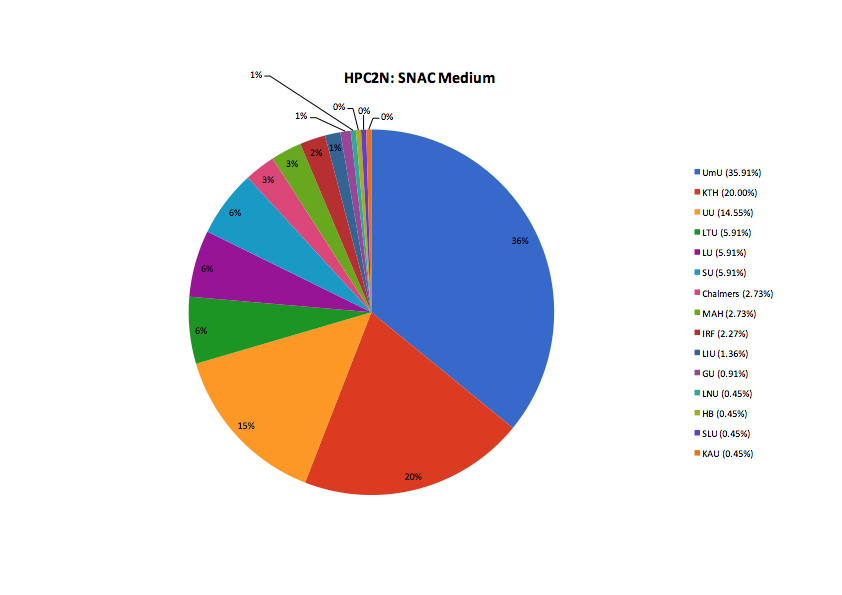
\includegraphics[width=0.9\textwidth]{figures/medium-users.png}
Projects with allocations at HPC2N: 2014-01-01 to 2016-05-30
\end{center}
}

\frame{
\frametitle{HPC2N (large users by university)}
\begin{center}
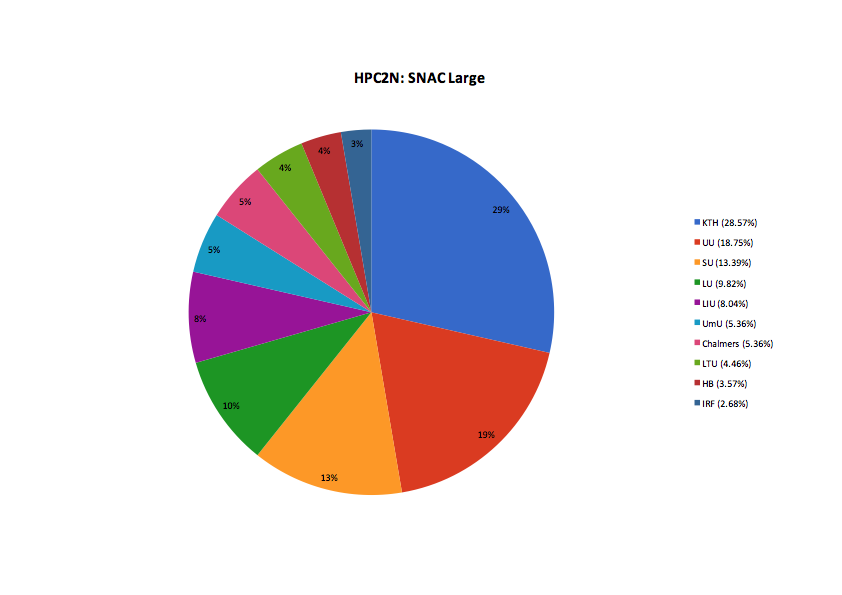
\includegraphics[width=0.9\textwidth]{figures/large-users.png}
Projects with allocations at HPC2N: 2014-01-01 to 2016-05-30
\end{center}
}

\frame{
\frametitle{HPC2N (users by software)}
\begin{center}
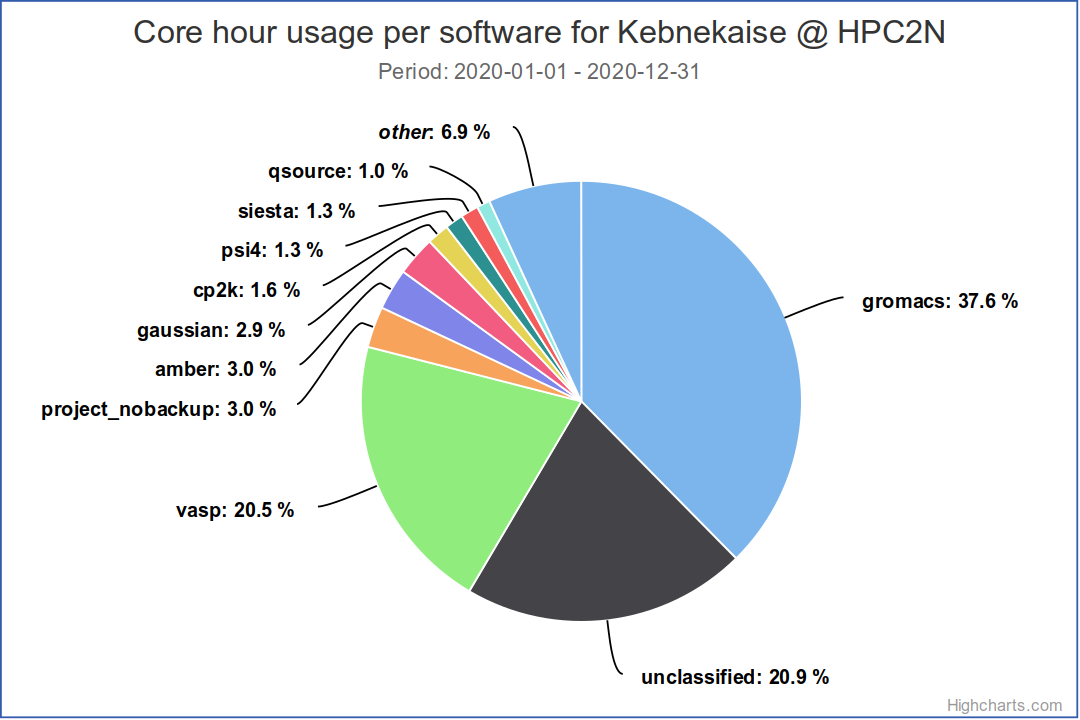
\includegraphics[width=0.9\textwidth]{figures/software.png}
\end{center}
}

\frame{
\frametitle{Kebnekaise}
\begin{itemize}
 \item \emph{Latest supercomputer at HPC2N}
 \pause \item Named after a massif (contains some of Sweden's highest mountain peaks)
 \pause \item Kebnekaise was 
 \begin{itemize}
  \item delivered by Lenovo and 
  \item \emph{installed during the summer 2016}
 \end{itemize}
 \pause \item Opened up for general availability on November 7, 2016
 \pause \item In 2018, Kebnekaise was \emph{extended} with 
 \begin{itemize}
  \item 52 Intel Xeon Gold 6132 (Skylake) nodes, as well as 
  \item 10 NVidian V100 (Volta) GPU nodes
 \end{itemize}
\end{itemize}
}

\frame{
\frametitle{Kebnekaise (compute nodes)}
\begin{tabular}{rcp{6.0cm}}
 Name & \# & Description \\ \hline 
        \color{cyan} Compute & \emph{432} & \makecell[l]{Intel Xeon E5-2690v4, \emph{2 x 14 cores}, \\\emph{128 GB}, FDR Infiniband} \\ \hdashline
 \pause \color{cyan} Compute-skylake & 52 & \makecell[l]{Intel Xeon Gold 6132, 2 x 14 cores, \\\emph{192 GB}, EDR Infiniband, \emph{AVX-512}} \\ \hdashline
 \pause \color{cyan} Large Memory & 20 & \makecell[l]{Intel Xeon E7-8860v4, \emph{4 x 18 cores}, \\\emph{3072 GB}, EDR Infiniband} \\ \hdashline
 \pause \color{cyan} KNL & 36 & \makecell[l]{Intel \emph{Xeon Phi} 7250 (Knight's Landing), \\ 68 cores, 192 GB, 16 GB MCDRAM, \\FDR Infiniband}
\end{tabular}
}

\frame{
\frametitle{Kebnekaise (GPU nodes)}
\begin{tabular}{rcp{7.0cm}}
 Name & \# & Description \\ \hline
        \color{cyan} 2xGPU & 32 & \makecell[l]{Intel Xeon E5-2690v4, 2 x 14 cores,\\ 128 GB, FDR Infiniband,\\ \emph{2 x NVidia K80} \\ 4 x 2496 CUDA cores, 4 x 12 GB VRAM} \\ \hdashline
 \pause \color{cyan} 4xGPU & 4 & \makecell[l]{Intel Xeon E5-2690v4, 2 x 14 cores,\\ 128 GB, FDR Infiniband,\\ \emph{4 x NVidia K80} \\ 8 x 2496 CUDA cores, 8 x 12 GB VRAM} \\ \hdashline
 \pause \color{cyan} GPU-volta & 10 & \makecell[l]{Intel Xeon Gold 6132, 2 x 14 cores,\\ 192 GB, EDR Infiniband, \\\emph{2 x NVidia V100}, \\2 x 5120 CUDA cores, 2 x 16 GB VRAM, \\\emph{2 x 640 Tensor cores}} \\
\end{tabular}
}

\frame{
\frametitle{Kebnekaise (in numbers)}
\begin{itemize}
 \item 602 nodes in 15 racks
 \pause \item \emph{19288 cores} (of which 2448 cores are KNL-cores)
 \begin{itemize}
  \item 18840 available for users (the rest are for managing the cluster)
 \end{itemize}
 \pause \item More than \emph{136 TB memory}
 \pause \item 71 switches (Infiniband, Access and Managment networks)
 \pause \item 728 TFlops/s Peak performance (expansion not included)
 \pause \item \emph{629 TFlops/s} Linpack (all parts, except expansion)
 \begin{itemize}
  \item 86\% of Peak performance
 \end{itemize}
\end{itemize}
}

\frame{
\frametitle{Kebnekaise (HPC2N storage)}
\begin{itemize}
 \item Basically five types of storage are available at HPC2N:
 \begin{itemize}
  \pause \item {\color{cyan} Home directory}
  \begin{itemize}
   \item \texttt{/home/X/Xyz}, \texttt{\$HOME}, \texttt{$\sim$}
   \item 25 GB, user owned
  \end{itemize}
  \pause \item {\color{cyan} Project storage}
  \begin{itemize}
   \item \texttt{/proj/nobackup/abc}
   \item Shared among project members
  \end{itemize}
  \pause \item {\color{cyan} Local scratch space}
  \begin{itemize}
   \item \texttt{\$SNIC\_TMP}
   \item SSD (170GB), per job, per node, "volatile"
  \end{itemize}
  \pause \item {\color{cyan} SweStore} --- disk based (dCache)
  \begin{itemize}
   \item part of SNIC Storage, \emph{nationally accessible storage}
  \end{itemize}
  \pause \item {\color{cyan} Tape Storage}
  \begin{itemize}
   \item Backup
   \item \emph{Long term storage}
  \end{itemize}
 \end{itemize}
\end{itemize}
}

\frame{
\frametitle{Kebnekaise (projects)}
\begin{itemize}
 \item In order to use Kebnekaise, you must be a member of a \emph{compute project}
 \begin{itemize}
  \pause \item A compute project has a certain number of \emph{core hours} allocated for it per month
  \pause \item A regular CPU core cost 1 core hour per hour, other resources (e.g., GPUs) cost more
  \pause \item Not a hard limit but projects that go over the allocation get lower priority
 \end{itemize}
 \pause \item A compute project contains a certain amount of storage
 \begin{itemize}
  \item If more storage is required, you must be a member of a \emph{storage project}
 \end{itemize}
% \pause \item Birgitte will cover more details
 \pause \item I will cover more details in the next section, where we
 go more in to detail about HPC2N and Kebnekaise 
\end{itemize}
}

\frame{
\frametitle{High Performance Computing (definition)}
\say{High Performance Computing most generally refers to the practice of \emph{aggregating computing power} in a way that delivers much \emph{higher performance} than one could get out of a typical desktop computer or workstation in order to \emph{solve large problems} in science, engineering, or business.}\footnote{https://insidehpc.com/hpc-basic-training/what-is-hpc/\\}
}

\frame{
\frametitle{High Performance Computing (opening the definition)}
\begin{itemize}
 \item \emph{Aggregating computing power}
 \begin{itemize}
  \item 602 nodes in 15 racks totalling 19288 cores
  \item Compared to 4 cores in a modern laptop
 \end{itemize}
 \pause \item \emph{Higher performance}
 \begin{itemize}
  \item 728\,000\,\underline{000}\,\underline{000}\,\underline{000} arithmetical operations per second\footnote{728 trillion (billion)}
  \item Compared to 200\,\underline{000}\,\underline{000}\,\underline{000} Flops in a modern laptop\footnote{200 billion (milliard)\\}
 \end{itemize}
 \pause \item \emph{Solve large problems}
 \begin{itemize}
  \item When does a problem become large enough for HPC?
  \item Are there other reasons for using HPC resources? (Memory,
    software, support, etc.) 
 \end{itemize}
\end{itemize}
}

\frame{
\frametitle{High Performance Computing (large problems)}
\begin{itemize}
 \item A problem can be large for two main reasons:
 \begin{enumerate}
  \item {\color{cyan} Execution time}: The time required to form a solution to the problem is very long
  \item {\color{cyan} Memory / storage use}: The solution of the problem requires a lot of memory and/or storage
 \end{enumerate}
 \pause \item The former can be remedied by \emph{increasing the performance}
 \begin{itemize}
  \item More cores, more nodes, GPUs, \dots
 \end{itemize}
 \pause \item The latter by \emph{adding more memory / storage}
 \begin{itemize}
  \item More memory per node (including large memory nodes), more nodes, \dots
  \item Large storage solutions, \dots
 \end{itemize}
\end{itemize}
}

\frame{
\frametitle{High Performance Computing (what counts as HPC)}
\begin{center}
 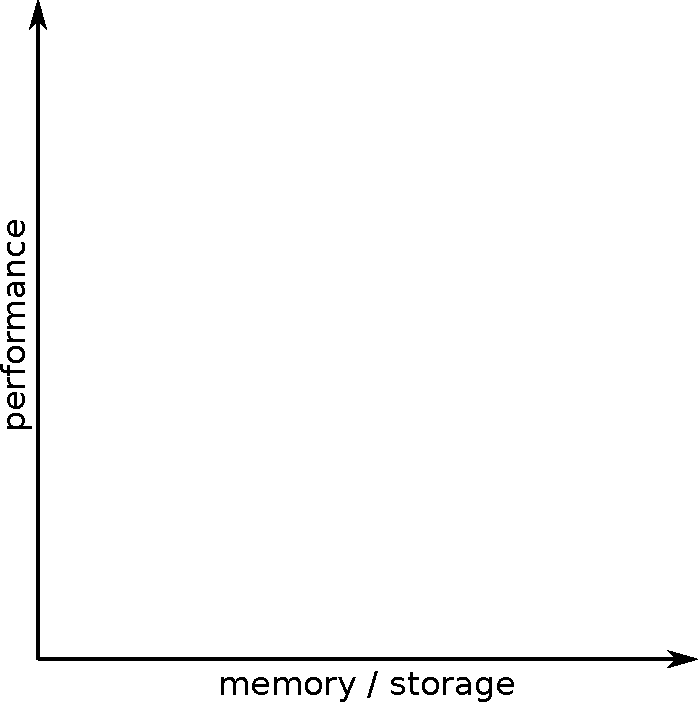
\includegraphics[width=0.6\textwidth]{figures/hpc1.pdf}
\end{center}
}

\frame{
\frametitle{High Performance Computing (what counts as HPC)}
\begin{center}
 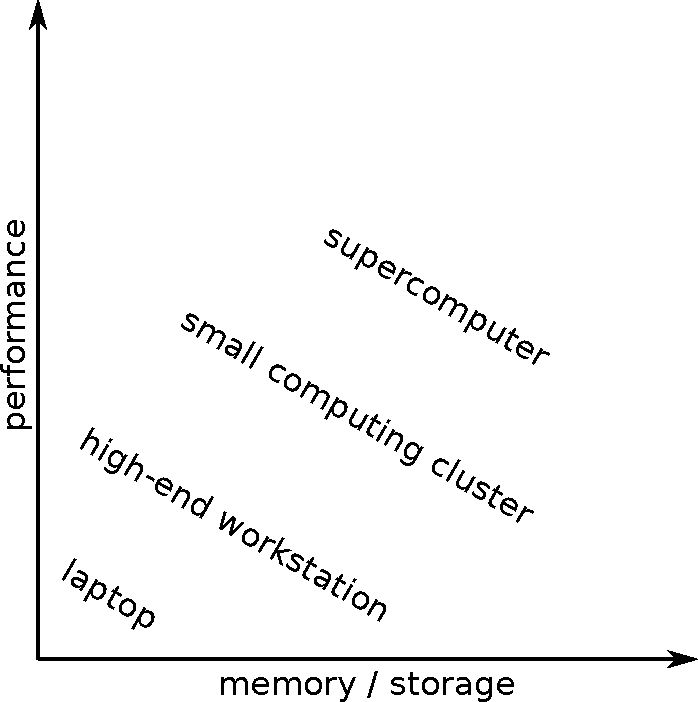
\includegraphics[width=0.6\textwidth]{figures/hpc2.pdf}
\end{center}
}

\frame{
\frametitle{High Performance Computing (what counts as HPC)}
\begin{center}
 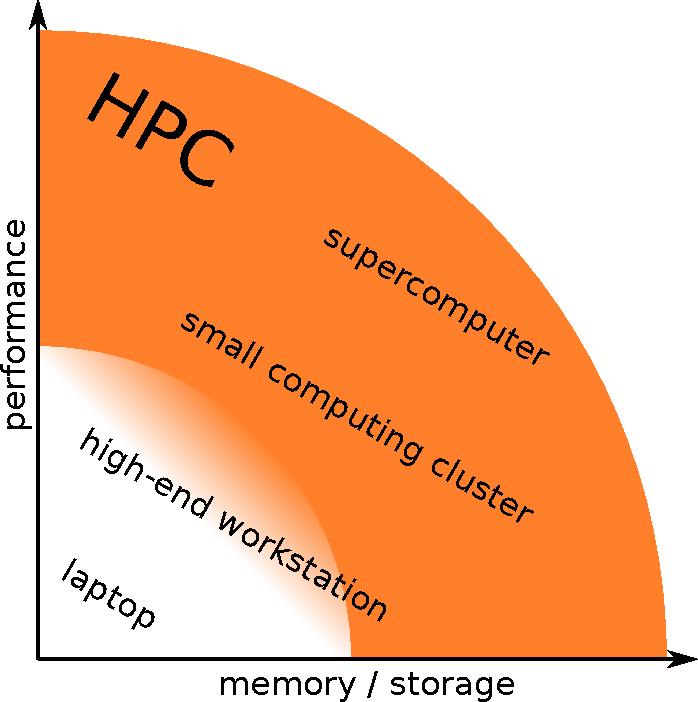
\includegraphics[width=0.6\textwidth]{figures/hpc3.pdf}
\end{center}
}

\frame{
\frametitle{High Performance Computing (other reasons)}
\begin{itemize}
 \item Specialized (expensive) hardware
 \begin{itemize}
  \pause \item GPUs, \emph{Nvidia Tesla V100 GPUs} are optimized for AI
  \pause \item Intel Xeon Phi
  \pause \item High-end CPUs (AVX-512 etc) and ECC memory
 \end{itemize}
 \pause \item Software
 \begin{itemize}
  \item HPC2N holds \emph{licenses} for several softwares
  \item Software is \emph{pre-configured and ready-to-use}
 \end{itemize}
 \pause \item \emph{Support and documentation}
\end{itemize}
}

\frame{
\frametitle{High Performance Computing (memory models)}
\begin{itemize}
 \item Two memory models are relevant for HPC:
 \begin{itemize}
  \pause \item {\color{cyan} Shared memory}: Single memory space for all data.
   \begin{minipage}{0.3\textwidth}
   \vspace{1mm}
   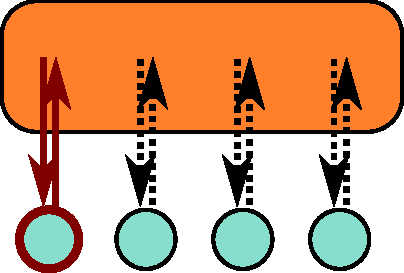
\includegraphics[scale=0.45]{figures/sm.pdf}
   \vspace{1mm}
  \end{minipage}\,
  \begin{minipage}{0.4\textwidth}
   \begin{itemize}
    \item \emph{Everyone can access the same data}
    \item Straightforward to use
   \end{itemize}
  \end{minipage}
  \pause \item {\color{cyan} Distributed memory}: Multiple \emph{distinct} memory spaces.
  \begin{minipage}{0.3\textwidth}
   \vspace{1mm}
   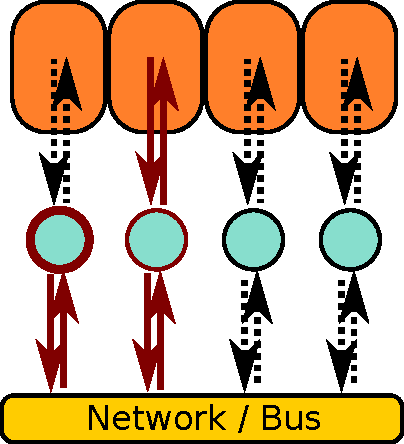
\includegraphics[scale=0.45]{figures/dm.pdf}
   \vspace{1mm}
  \end{minipage}\,
  \begin{minipage}{0.4\textwidth}
   \begin{itemize}
    \item Everyone has direct access \emph{only to the local data}
    \item Requires \emph{communication}
   \end{itemize}
  \end{minipage}
 \end{itemize}
\end{itemize}
}

\frame{
\frametitle{High Performance Computing (memory models)}
\begin{center}
 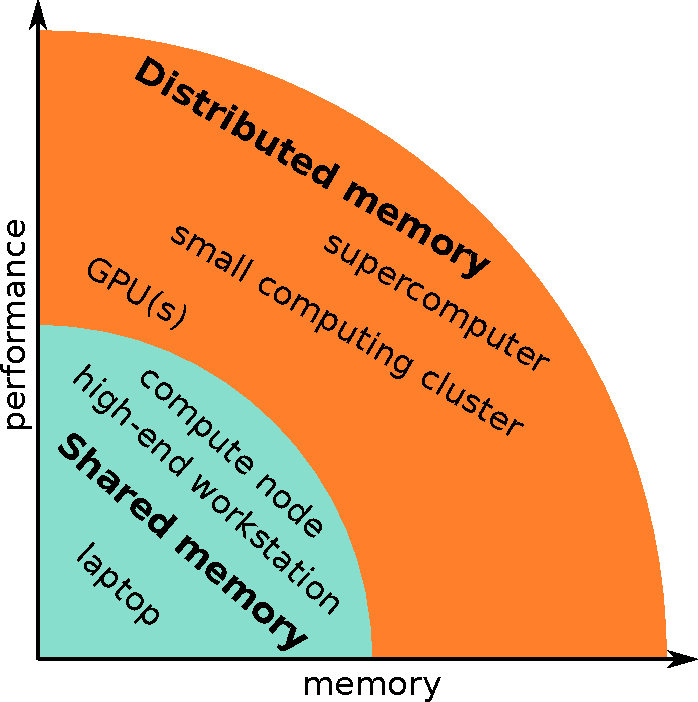
\includegraphics[width=0.6\textwidth]{figures/memory.pdf}
\end{center}
}

\frame{
\frametitle{High Performance Computing (programming models)}
\begin{itemize}
 \item The programming model changes when we aim for extra performance and/or memory:
 \begin{enumerate}
  \pause \item {\color{cyan} Single-core}: Matlab, Python, C, Fortran, \dots
  \begin{itemize}
   \item Single stream of operations
  \end{itemize}
  \pause \item {\color{cyan} Multi-core}: Vectorized Matlab, pthreads, \emph{OpenMP}
  \begin{itemize}
   \item \emph{Multiple streams} of operations
   \pause \item \emph{Work distribution}, \emph{coordination} (synchronization, etc), \dots
  \end{itemize}
  \pause \item {\color{cyan} Distributed memory}: \emph{MPI}, \dots
  \begin{itemize}
   \item Multiple streams of operations
   \item Work distribution, coordination (synchronization, etc), \dots
   \pause \item \emph{Data distribution and communication}
  \end{itemize}
 \end{enumerate}
 \pause \item {\color{cyan} GPUs}: \emph{CUDA}, OpenCL, OpenACC, OpenMP, \dots
 \begin{itemize}
  \pause \item \emph{Many lightweight} streams of operations
  \pause \item Work distribution, coordination (synchronization, etc), \dots
  \pause \item \emph{Data distribution across memory spaces and movement}
 \end{itemize}
\end{itemize}
}

\frame{
\frametitle{High Performance Computing (software)}
\begin{itemize}
 \item Complexity grows when we aim for extra performance and/or memory/storage:
 \begin{enumerate}
  \pause \item {\color{cyan} Single-core}: LAPACK, \dots
  \begin{itemize}
   \item Load correct toolchain etc
  \end{itemize}
  \pause \item {\color{cyan} Multi-core}: LAPACK + parallel BLAS, \dots
  \begin{itemize}
   \item Load correct toolchain etc
   \pause \item \emph{Allocate} correct number of cores, \emph{configure} software to use correct number of cores, \dots
  \end{itemize}
  \pause \item {\color{cyan} Distributed memory}: ScaLAPACK, \dots
  \begin{itemize}
   \item Load correct toolchain etc
   \pause \item Allocate correct number of \emph{nodes and cores}, configure software to use correct number of \emph{nodes and cores}, \dots
   \pause \item Data distribution, storage, \dots
  \end{itemize}
 \end{enumerate}
 \pause \item {\color{cyan} GPUs}: MAGMA, TensorFlow, \dots
 \begin{itemize}
  \item Load correct toolchain etc
  \item Allocate correct number of \emph{cores and GPUs}, configure software to use correct number of \emph{cores and GPUs}, \dots
 \end{itemize}
\end{itemize}
}

\frame{
\frametitle{End (questions?)}
\centering \Huge Questions?
}


\end{document}
